%%%%%%%%%%%%%%%%%%%%%%%%%%%%%%%%%%%%%%%%%%%%%%%%%%%%%%%%%%%%%%%%%%%%%%%%%%%%%%
%%% Sample file for MTech Project Papers for Evaluation by Supervisor and Reader
%%Skeleton LaTeX file: double column format.
%%%%%%%%%%%%%%%%%%%%%%%%%%%%%%%%%%%%%%%%%%%%%%%%%%%%%%%%%%%%
%%REMEMBER  THE PAGE SIZE RESTRICTIONS
%%Mid-term :   8 Pages
%%Final        : 16 Pages
%%%%%%%%%%%%%%%%%%%%%%%%%%%%%%%%%%%%%%%%%%%%%%%%%%%%%%%%%%%%


\documentclass{article}
\usepackage{hyperref}
\usepackage[numbers]{natbib}
\usepackage{mathtools}
\DeclarePairedDelimiter\floor{\lfloor}{\rfloor}
\usepackage{multicol}





\usepackage{graphicx,changepage}
\usepackage{amsmath}
\usepackage{caption}
\graphicspath{ {images/} }
\pagestyle{empty}
\setlength{\topmargin}{ 0.25in}
\setlength{\columnsep}{2.0pc}
\setlength{\headheight}{0.0in}
\setlength{\headsep}{0.0in}
\setlength{\oddsidemargin}{-.19in}
\setlength{\parindent}{1pc}
\textheight 8.75in
\textwidth 6.8in
\newcommand{\quotes}[1]{``#1''}
\title{\large \bf Moving beyond RNNs: Attention Networks }
\author{Sachin Mittal}

\date{}

\begin{document}

	\maketitle
    \begin{center}
        Mid-term MTech Project Report
    \end{center}
        \vskip 12pt
	\thispagestyle{empty}
	\bibliographystyle{unsrt}
	
		\begin{abstract}
		RNNs are very common in any sequence to sequence task and have an inherently serial structure that prevents them from being run in parallel. RNNs are not invariant to the distance between tokens, i.e. as the distance grows between input tokens, it becomes harder to capture the dependencies between them. In this report, We study a new simple network architecture, the Transformer, based solely on attention mechanisms, and entirely dispensing with recurrence and convolutions. Transformer \cite{DBLP:journals/corr/VaswaniSPUJGKP17} was released one year back (2017) by Google team and has shown state of the art result at that time on two machine translation tasks. Despite achieving state of art result, it fails to generalize in many tasks (e.g. copying strings or even simple logical inference when the string or formula lengths exceed those observed at training time), however, those tasks can be handled by RNNs with ease. 
         In the later section, we have described a recently proposed architecture by Google team namely, Universal Transformer\cite{dehghani2018universal}. Experiments in the original paper show that  Universal Transformer is able to generalize on various algorithmic tasks and language understanding tasks. UT outperforms both Transformer and LSTM in machine translation and also achieves the new state of the art on the bAbI linguistic reasoning task\cite{weston2015aicomplete}.
	\end{abstract}	
	
	\hfill \\
	
	\begin{multicols}{2}
	\section{INTRODUCTION}
The sequence to sequence learning has been successful in many tasks such as machine translation, speech recognition, and text summarization etc. A typical Encoder-Decoder model encodes the input sequence with a series of bi-directional recurrent neural networks (RNNs) and generates variable length output with another set of decoder RNNs, both of which interface via a soft-attention mechanism.
Traditionally, both the encoder and the decoder were composed of recurrent neural networks (RNNs). RNNs sequentially process the input tokens $(x_1, x_2, ... , x_n)$  into hidden encoding $(z_1, z_2, ... , z_n)$ , then sequentially generate the output tokens $(y_1, y_2, ... , y_m)$. There are two main problems with this approach.

First is the sequential nature of RNNs. $z_i$  depends on $z_{i-1}$ , meaning it is impossible to compute $z_i$  and $z_{i-1}$  in parallel. The ability to process inputs in parallel is very important in deep learning since we normally use GPUs which work far better for parallel inputs. The other is the difficulty of learning long-range dependencies in the network. 
\\ In this report, we mainly present three architectures-  Transformer, Universal Transformer, and Semi-Autoregressive transformer. All architectures rely entirely on an attention mechanism to draw global dependencies between input and output and allows significantly more parallelization. The later two architectures have Transformer as the base model and modified it to some extent. We have presented the Transformer in detail, that will also enable us to explain how the later two architectures are working with Transformer as a base model.
		
	\section{Transformer}
The Transformer $-$ A model that completely rely on attention to increase the training speed of the model. To illustrate details about Transformer we have used machine translation as an example.


\begin{center}
\captionsetup{type=figure}
        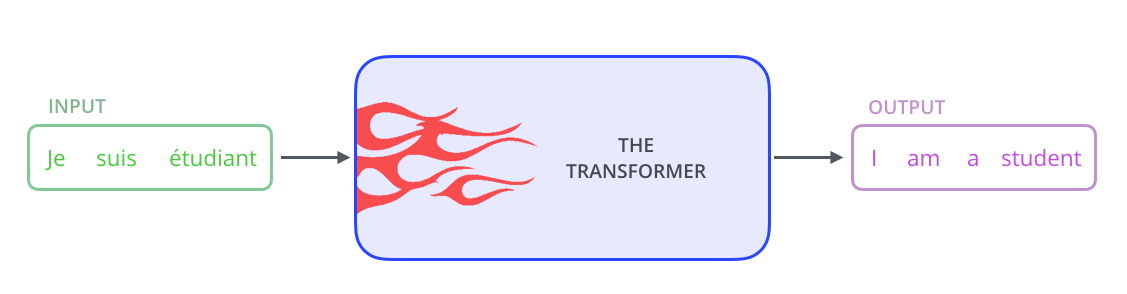
\includegraphics[width=.47\textwidth]{the_transformer_blackbox.png}
        \captionof{figure}{Transformer as black box for machine translation }
\end{center}

Transformer is encoder-decoder architecture unlike traditional encoder-decoders It attends all of the input in parallel.

\begin{center}
        \captionsetup{type=figure}
        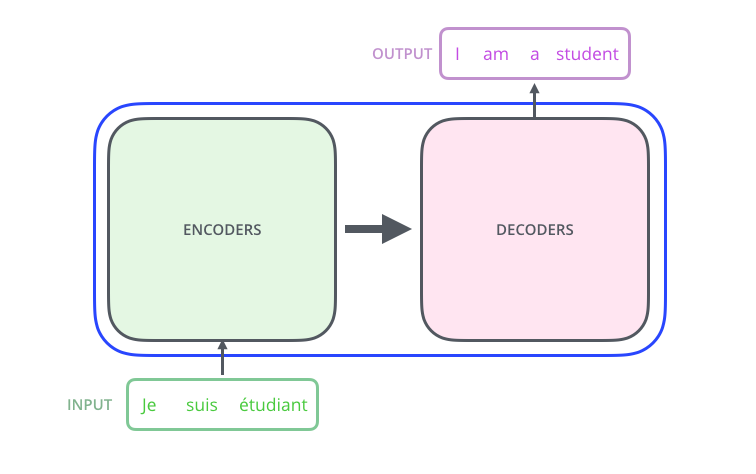
\includegraphics[width=.40\textwidth]{2.png}
        \captionof{figure}{Transformer: Encoder-Decoder }
\end{center}

Both components (encoding and decoding) are the stack of $N$ identical encoder(decoder) on top of each other. \\  \textbf{Encoder} consists of two sublayers namely, self-attention and feedforward. Each of these sublayer has layer-normalization step and residual connections before passing it to the subsequent layer.

Below figure shows that how sublayers in one of the encoders (out of $N$ stacked encoders) interacts each other.

\begin{center}
        \captionsetup{type=figure}
        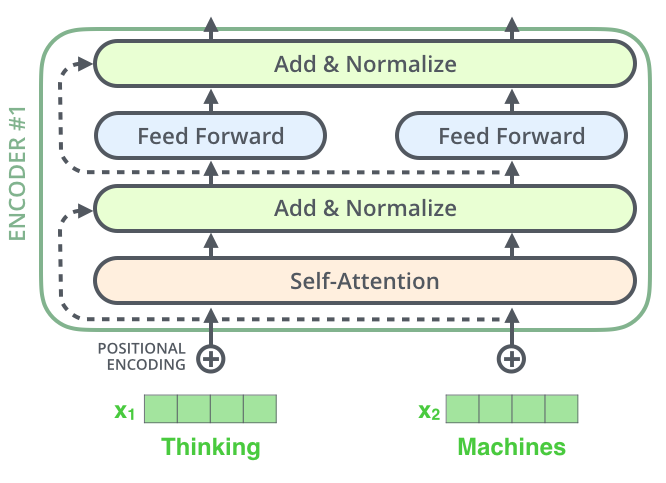
\includegraphics[width=.40\textwidth]{EncoderSublayer.png}
        \captionof{figure}{Encoder Sublayers and their interaction}
          \label{encoderSublayer}
\end{center}

Figure~\ref{encoderSublayer} depicts that input to the encoder first passed through Self Attention layer then to Feed Forward layer. The output from Feed Forward layer passes to subsequent encoders.


 \subsection{Self Attention}
 The first step in calculating self-attention is to create three vectors using the input of the encoder. The very first encoder has the embedding of words as input and later encoders (in stacked encoders) has the output of the previous encoder as input to themselves. To generate three vectors - query, key and value, We have three (trainable) matrices $W^Q$, $W^K$ and  $W^V$.
 Multiplying $x_1$ with weight matrix $W^Q$ produces $q_1$, the "query" vector associated with that word. Similarly, we end up creating a "query", a "key", and a "value" vectors for each input word which is a linear projection of each word.

\begin{center}
       $q_i = x_iW^Q$ \\
        $k_i = x_iW^K$\\
         $v_i = x_iW^V$
       
\end{center}
After finding out these three vectors, we are all set to calculate self-attention scores. The score determines how much to focus on other parts of the input sentence as we encode a word at a certain position. The reason why it is called self-attention is that we compare each word with its own too.

\noindent To calculate scores for $i^{th}$ word, we need to compare it against every word in sequence. We take query vector of $i^{th}$ word and key vectors of every other word and perform dot product. These dot products are supplied to softmax and later gets multiplied with value vectors.
\begin{center}
       $e_{ij} = \frac{1}{\sqrt{d_k}}(q_i)(k_j)^T$
   \end{center}
   
   
\begin{center}
        \captionsetup{type=figure}
        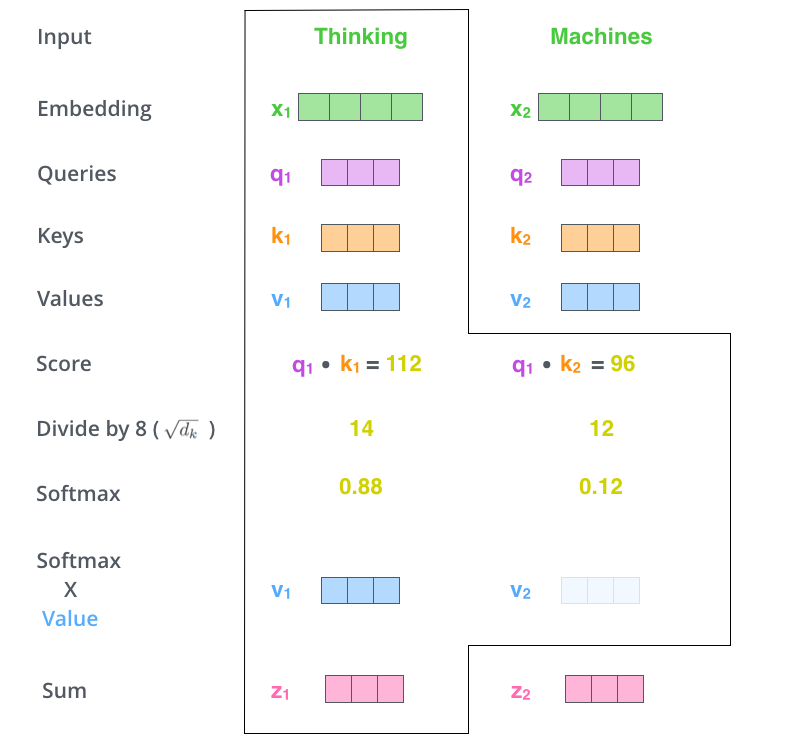
\includegraphics[width=.40\textwidth]{ZvectorSoftmax.png}
        \captionof{figure}{Attention calculation (here $z_1 =  (0.88 \times v_1) + (0.12 \times v_2)$) }
\end{center}


\noindent Since we can deal with matrices, so we can condense all calculations of $z$ vectors into matrix form- 
\begin{center}
$Z = \text{softmax}\Big( \frac{Q\times K^T}{\sqrt{d_k}} \Big)V$\\
\end{center}
where $d_k$ is the dimension of the key. The authors scale the dot product by $1/\sqrt{d_k}$ to avoid the
inputs to softmax function growing too large in magnitude.
\subsection{The core component: Multi-Head Attention}
Instead of using single attention head, Transformer uses multiple attentions with different linear transformation. Doing this, Transformer captures various relationship among different words which was not possible with single head attention.  
Further, it reduces the number of operations to capture the relation between two words in a sequence to $O(1)$ whereas it takes O(n) for ConvS2S \cite{DBLP:journals/corr/GehringAGYD17} and O(logn) for ByteNet \cite{DBLP:journals/corr/KalchbrennerESO16}.
Multi-Head Attention calculates multiple attention weighted sums $–$ hence the name \quotes{Multi-Head} Attention.

Multi-Head Attention applies different linear transformations to the values, keys, and queries for each \quotes{head} of attention. This is illustrated in the following figure:
\begin{center}
        \captionsetup{type=figure}
        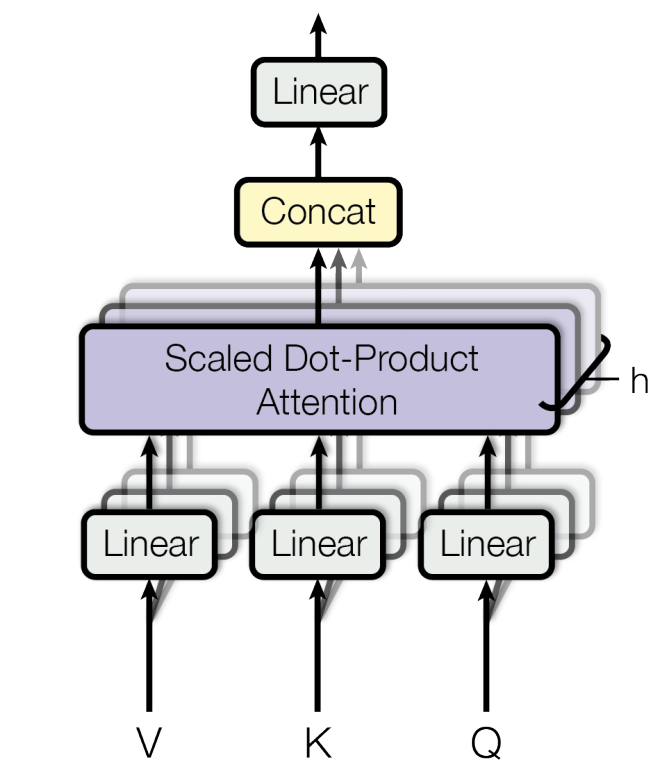
\includegraphics[width=.40\textwidth]{MultiHead.png}
        \captionof{figure}{MultiHead Attention (where $h$ is number of \quotes{heads}) }
         \label{multiHead} 
\end{center}

Multihead Attention results in multiple $Z$ matrices but sublayer2 (Feedforward layer) in the encoder is expecting only one $Z$ matrix. We concatenate them and again perform linear projection with (trainable) weight matrix $W^O$. Figure~\ref{multiHead} describes the overall picture, that can also be written mathematically using following equation -
\begin{center}
$\text{MultiHead}(Q, K, V ) = \text{Concat} (Z_1, Z_2 \dots Z_h)W^O$
where $Z_i = \text{Attention} (XW^Q_i,XW^K_i, XW^V_i)$\\
and $X$ is input to encoder.
\end{center}


\subsection{Preserving The Order of The Sequence Using Positional Encoding}
Since we are dealing with sequential data, we need to take care of sequence in which the words are. For this purpose, the Transformer uses Positional Encodings. Positional encodings explicitly encode the relative/absolute positions of the inputs as vectors and are then added to the input embeddings.
Following equations are used to compute the positional encodings:
\begin{center}
$\text{PE(pos,2i) = sin(pos/10000}^{2i/d_{model}})$\\
$\text{PE(pos,2i+1) = cos(pos/10000}^{2i/d_{model}})$
\end{center}
\noindent The idea here is that adding these values to the embeddings provides meaningful distances between the embedding vectors once they’re projected into Q/K/V vectors and during dot-product attention.
Positional embeddings are only added to the input of the first encoder, later encoders have previous encoder outputs as input.

\subsection{Feed-Forward layer (Sublayer2)}
The output of attention sublayer is fed to Feed-Forward layer. Attention sublayer encodes each word $x_i$ in input sequence to $z_i$ which gets passed to Feed-Forward networks(see Figure~\ref{encoderOutputs}). Feed-Forward layer operation can be seen as follows:- 

\begin{center}
$FFN(z) = max(0, zW_1 + b_1)W_2 + b_2$
\end{center}

\begin{center}
        \captionsetup{type=figure}
        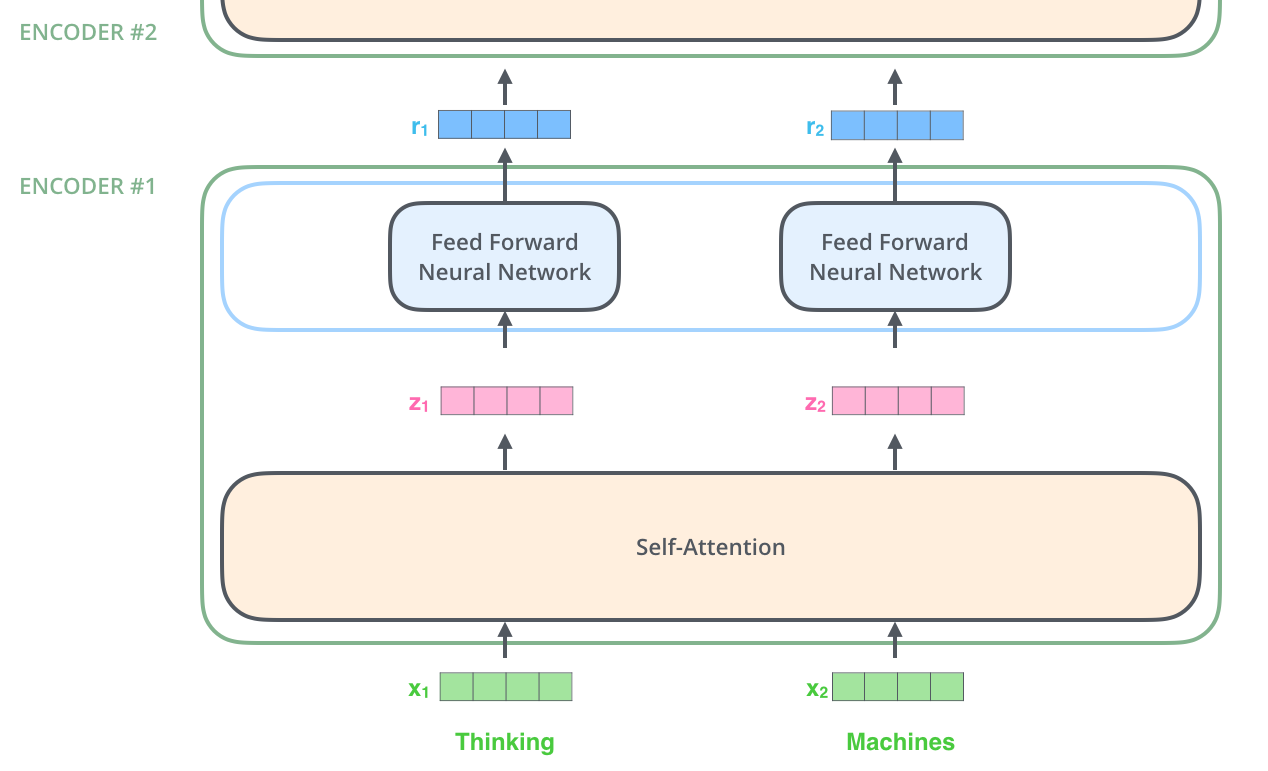
\includegraphics[width=.40\textwidth]{encoderOutputs.png}
        \captionof{figure}{The word at each position passes through a self-encoding process. Then, they each pass through a feed-forward neural network }
         \label{encoderOutputs} 
\end{center}

\noindent We apply the fully connected layer to each position separately and identically. This consists of two linear transformations with a ReLU activation in between.\\


\noindent Here $W_1, b_1,W_2 \text{ and } b_2$  are shared among all words in sequence. This operation can be viewed as 1D convolution operation on sequence.

\subsection{Decoder}

The decoder is very similar to the encoder but has one additional sub-layer, which is a modification of the Multi-Head Attention network, called the “masked multi-head attention” network  (Figure~\ref{decoder}). 
The output of the top encoder is transformed into a set of attention vectors K and V. The attention vectors K and V have information about all positions of the input sequence. Attention sublayer in each decoder uses K and V, which helps the decoder focus on appropriate places in the input sequence. 
\begin{center}
        \captionsetup{type=figure}
        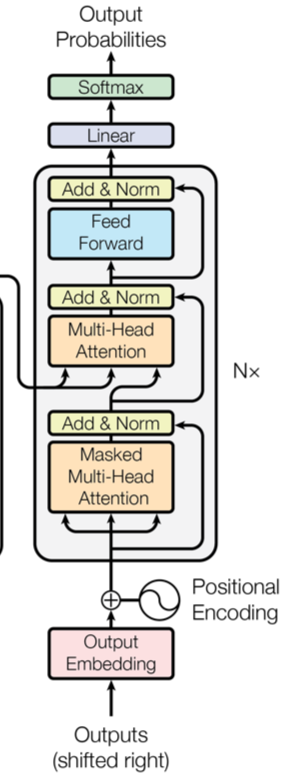
\includegraphics[height=.65\textwidth , width=.40\textwidth]{decoder.png}
        \captionof{figure}{Decoder }
        \label{decoder}
\end{center}


\noindent \textbf{Masked multi-head attention} layer is added to the decoder to prevent decoder to attend subsequent words which are not shown at output yet. Since at training time we know the ground truth (output at decoder side) but we are not supposed to use $y_{i+1}$ while producing $y_i$ in output. Moreover, While producing $y_{i+1}$, previously generated outputs $y_1, y_2 \dots y_i$ are fed to bottom most decoder with positional encodings (just like the way encoder does).
%%%%%%%%%%%%%  This can be followed by several other sections
    \section{Universal Transformer}
     Universal Transformers, an extension to standard Transformer which is computationally universal that combines advantages of both worlds, i.e. parallelization of Transformer and recurrence of RNNs.
     \\
     UT keeps the parallel structure of the Transformer but replaces fix sized stacked encoders(or decoders) with the recurrent transformation function. The word "recurrent" is there because same learned transformation function is applied to all symbols in parallel, where the output of the previous step is fed to input for the next step. Hence UT attends all input symbol in parallel (like transformer) but in each step iteratively refines its representations for all positions in the sequence parallelly (Figure~\ref{UTReccur}) .\\
     At first sight, it seems to restrict UT to apply same transition function repeatedly especially when compared to the standard Transformer which learns to apply a fixed sequence of distinct functions. But the recurrent function evolves per-symbol hidden states in parallel, and the number of processing steps can be variable. This is called \textbf{parallel in time recurrence mechanism} which process all inputs in parallel (unlike serial recurrence used in RNNs) and also boost up accuracy compared to vanilla Transformer. \\
     
  \noindent   Figure~\ref{UT} shows the overall architecture of Universal Transformer with position and step embeddings as well as dropout and layer normalization.

\begin{center}
\noindent \resizebox{1\hsize}{!}{
$\text{MultiHeadSelfAtttention}(H) = \text{Concat} (\text{head}_1, \text{head}_2 \dots \text{head}_k)W^O$}

where $\text{head}_i = \text{Attention} (HW^Q_i,HW^K_i, HW^V_i)$
\end{center}

At step t, the Universal Transformer computes revised representations $H^t \in  R^{m\times d}$ for all $m$ input positions as follows

\begin{center}
$H^t  = \text{LayerNorm}(A^{t-1})+\text{Transition}(A^t)$
 \noindent \resizebox{1\hsize}{!}{$ A^t  = \text{LayerNorm}(H^{t-1})+\text{MultiHeadSelfAttention}(H^{t-1}+P^t)$}
\end{center}

\noindent Depending on the task, Transition function is either feedforward network (similar to Transformer) or a separable
convolution. \\
$P^t$ above are two-dimensional (position, time) coordinate embeddings,

\begin{center}
$P^t_{\text{pos},2j} = sin(pos/10000^{2i/d})\bigoplus sin(t/10000^{2i/d})$
$P^t_{\text{pos},2j+1} = cos(pos/10000^{2i/d})\bigoplus cos(t/10000^{2i/d})$
\end{center}

After T steps, the final output of the Universal Transformer encoder is a matrix of d-dimensional vector representations $H^T \in  R^{m\times d}$ for the m symbols of the input sequence.


\begin{center}
        \captionsetup{type=figure}
        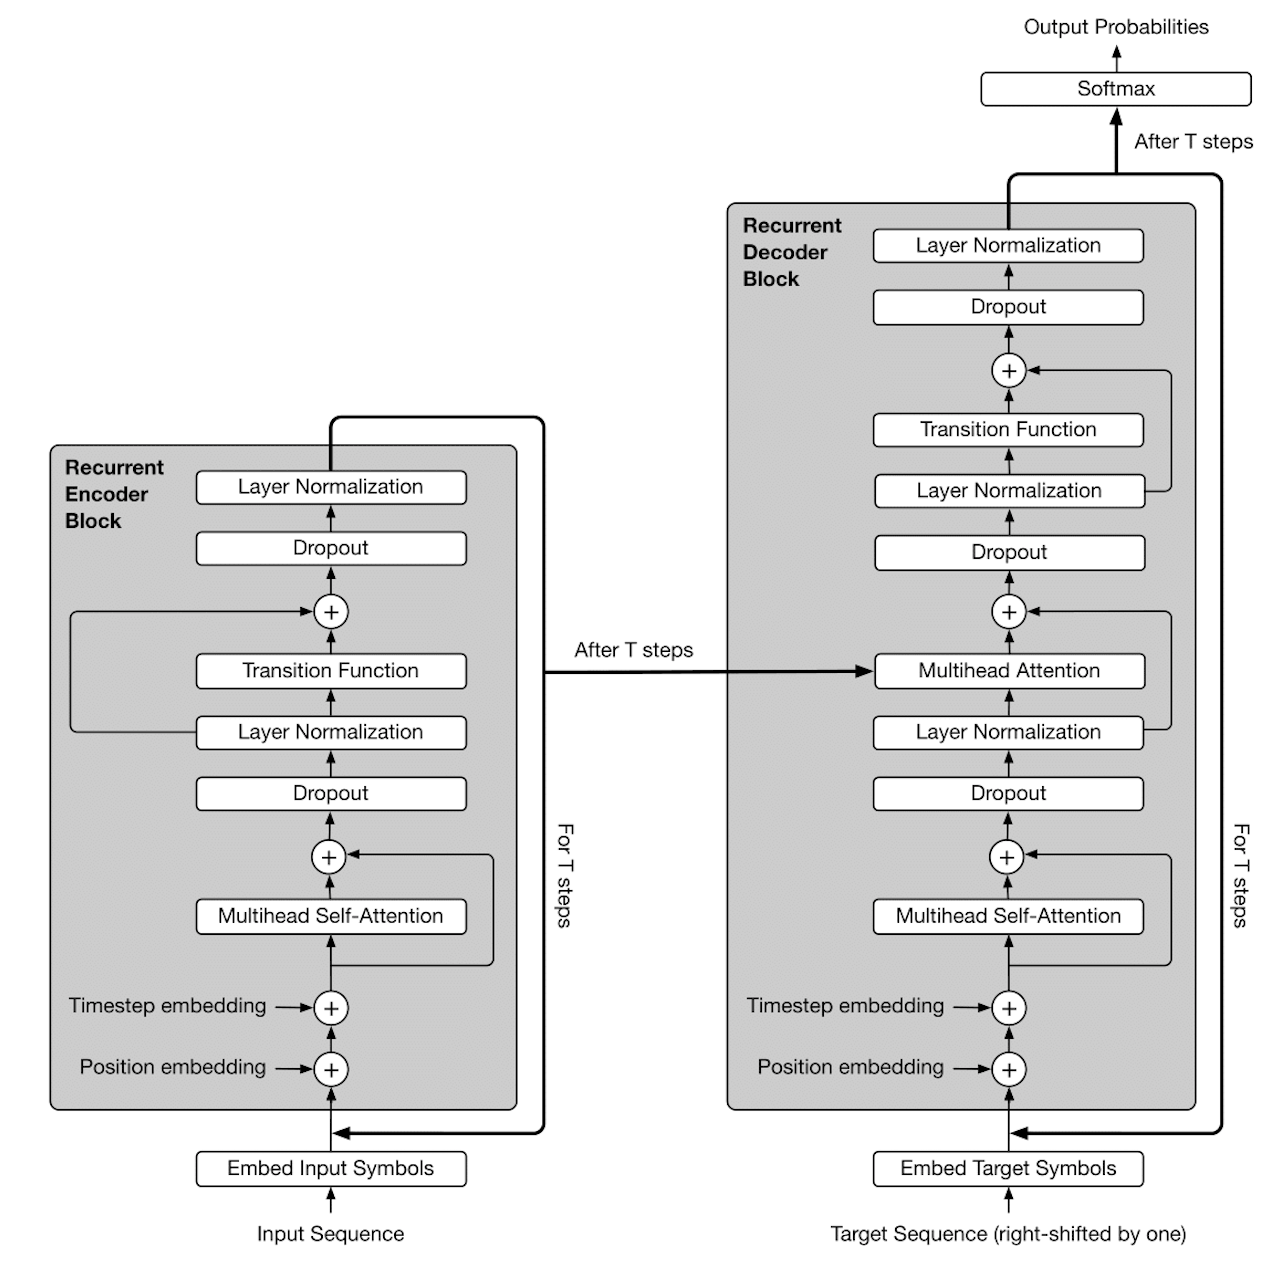
\includegraphics[height=.70\textwidth , width=.40\textwidth]{universal.png}
        \captionof{figure}{Universal Transformer }
        \label{UT} 
\end{center}
     
\begin{figure*}[ht]
\centering
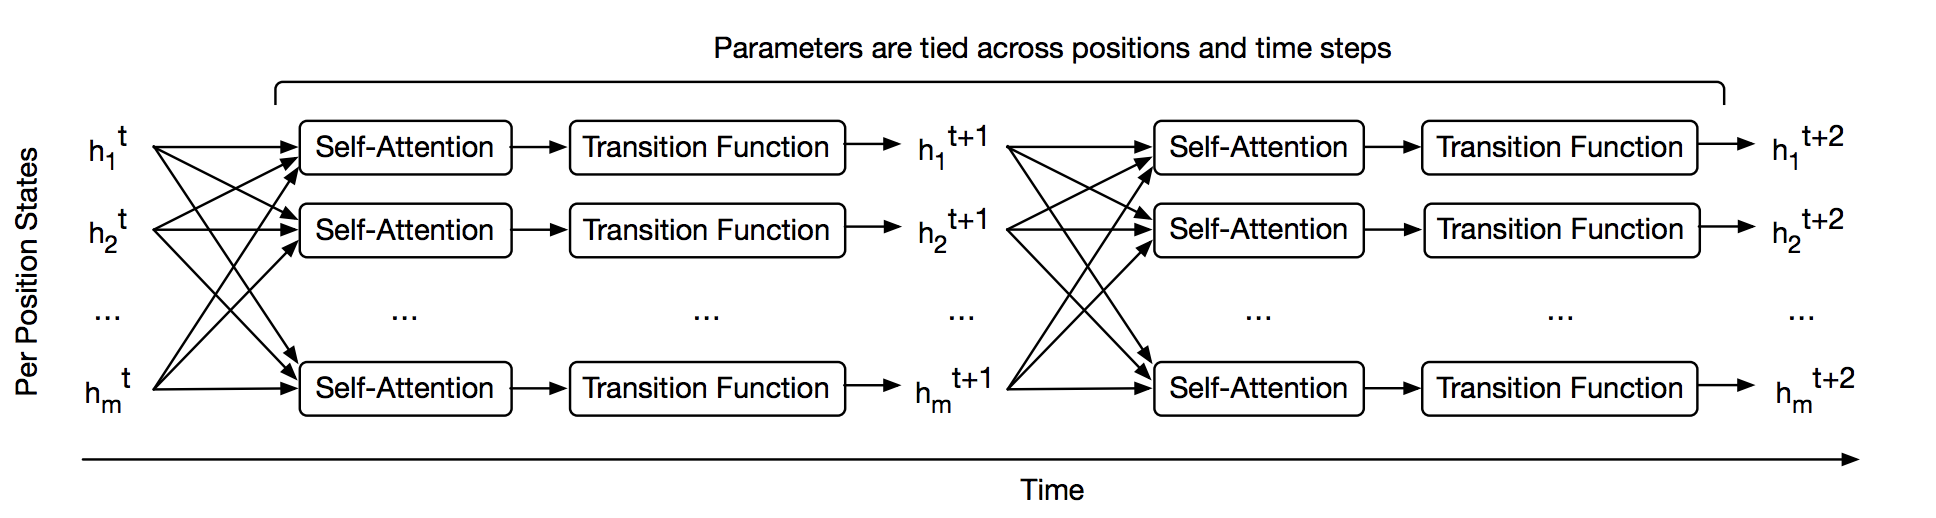
\includegraphics[ width=1\textwidth]{UTTime.png}
        \captionof{figure}{Universal Transformer with two recurrent steps }
        \label{UTReccur} 
\end{figure*}


\textbf{Decoder} is same as encoder except that it attends final encoder representation $H^T$ using the same multi-head dot-product attention with query $Q$ obtained from decoder input representation and key, value pair $K, V$ using the linear projection of $H^T$.\\
In sequence processing systems, few symbols are ambiguous than others. Consider the sentence \quotes{I arrived at the bank after crossing the river}. Here word \quotes{bank} is more ambiguous compared to other words hence it is reasonable to spend more processing resources for some words. Standard Transformer applies the same amount of processing to every word, unlike Universal Transformer. \\
Universal Transformer uses Adaptive Computation Time (ACT) \cite{DBLP:journals/corr/Graves16} mechanism to dynamically decide the number of processing steps required to process input words in sequence. \\
Universal Transformer increases theoretical expressibility of Transformer and makes it Turing complete.
UT achieves the new state of the art result on babI question answering task and  LAMBADA Language Modeling.
     \section{Semi-Autoregressive Transformer }   
    Transformers are auto-regressive, In the sense that they produce output one by one. 
    Semi-Autoregressive Transformer (SAT)\cite{wang2018semiautoregressive} keeps the autoregressive property in global but relieves in local and thus are able to produce multiple successive words in parallel at each time step. SAT achieves a good balance between accuracy and speed. On WMT’14
English-German translation, the SAT achieves
5.58× speedup while maintaining 88\% translation
quality. \\
SAT can produce $K$ words at a time (which is adjustable). Transformer can be viewed as a special case of Semi-Autoregressive Transformer when $K=1$. \\
   
\noindent Fundamental idea that SAT uses is, it groups the dependencies i.e. it extends word-level chain rule to the group-level chain rule.
 Any encoder-decoder architecture first encodes source sentence $x_1, x_2 \dots x_m$ into hidden states and then decoder generates target sentence $y_1, y_2 \dots y_n$  according to an autoregressive model 
$p(y_t|y_1, y_2 \dots y_{t-1}, \textbf{x})$. \\
Below factorization captures the idea behind group level chain rule.\\
  \noindent $p(y_1, y_2 \dots y_n \mid \textbf{x}) = {\displaystyle \prod_{t=1}^\floor*{\frac{(n-1)}{K}}+1} p(G_t|G_1, G_2 \dots G_{t-1}, \textbf{x}) $

    \noindent \resizebox{1\hsize}{!}{$G_1, G_2 \dots G_{\floor*{(n-1)/K}+1} = y_1, \dots y_k, y_{k+1} \dots y_{2k}, \dots y_{\floor*{(n-1)/K}\times K+1} \dots y_n$}
Here words in same group are independent and can be produced in parallel. \\
This way, SAT is able to perform long distance prediction.

\section{Self-Attention with Relative Position Representations}
Transformer uses absolute
positions to its input for positional encoding. Recent work by Shaw et al. \cite{shaw2018selfattention}(One of the authors of this paper is the first author for Transformer paper )  shows that we can modify transformer to capture relative position representation for the self-attention mechanism.
\\
Here We have revised Self-Attention mechanism used in Transformer followed by Relation aware self-attention, that is proposed mechanism to improve Transformer accuracy.
\begin{itemize}
    \item Self-Attention: \\
   Input sequence  $(x_1, x_2, ... , x_n)$ is passed through sublayers of encoder and mapped to  $(z_1, z_2, ... , z_n)$.
   \begin{center}
       $e_{ij} = \frac{1}{\sqrt{d_z}}(x_iW^Q)(x_jW^K)^T$
   \end{center}
   attention weight (alpha) is computed by softmax function-
    \begin{center}
      $\alpha _{ij} = \frac{\text{exp}e_{ij}}{\sum_{k=1}^{n} \text{exp}e_{ik}}$
   \end{center}
   These scores further gets multiply with \textbf{value} vectors to produce final token representation-
       \begin{center}
      $z_i = \sum_{j=1}^{n} \alpha _{ij}(x_jW^V)$
   \end{center}
   
   \item Relation aware self-attention:- \\
   Shaw et al. \cite{shaw2018selfattention} proposed relation aware self-attention in which edge information is added while keeping input and output same as Transformer.
    \begin{center}
       $e_{ij} = \frac{1}{\sqrt{d_z}}(x_iW^Q)(x_jW^K+a_{ij}^K)^T$
   \end{center}
  $\Big( \alpha _{ij}$ is same softmax function  $\alpha _{ij} = \frac{\text{exp}e_{ij}}{\sum_{k=1}^{n} \text{exp}e_{ik}}\Big)$ \\
  
  \noindent And final token representation is calculated using edge information too.
   \begin{center}
      $z_i = \sum_{j=1}^{n} \alpha _{ij}(x_jW^V+a_{ij}^V)$
   \end{center}
   maximum relative position is clipped to a max absolute value of k
 \begin{center}
      $ a_{ij}^K = w_{\text{clip}(j-1,k)}^K$\\
       $ a_{ij}^V = w_{\text{clip}(j-1,k)}^V$\\
       $ \text{clip}(x,k) = max(-k, min(k,x))$
   \end{center}
   On the WMT 2014 English-to-German and English-to-French translation tasks, this approach yields improvements of 1.3 BLEU and 0.3 BLEU over absolute position representations(Transformer), respectively.
\end{itemize}

\section{Work Planned and Future work}
I would first reproduce the results of Transformer using training tips in given in paper \cite{DBLP:journals/corr/abs-1804-00247}. After reproducing the existing results, I would test my model on different natural language generation tasks like Question-Answering. Further, I will test different possible positional encodings in Transformer to check if it boosts accuracy significantly. \\
In Future, I would first reproduce Universal Transformer results and then will replace positional encodings by encodings suggested for Transformer by Shaw et al. \cite{shaw2018selfattention}.
The final goal of this MTech project is to make Universal Transformer work in various Natural Language Tasks.
    \bibliography{refere}
    
    \bibliographystyle{abbrv}
    
    \end{multicols}
\end{document}
